\chapter{Literature Review}


\section{Sloan Digital Sky Survey (SDSS)} \label{sec:sectionsdss}

The Sloan Digital Sky Survey (SDSS) is a large scale multi spectral imaging and spectroscopic redshift survey using a dedicated 2.5 meter wide-angle optical telescope at Apache Point Observatory in New Mexico, USA. It began its operation in the year 2000 and since then have been taking continuous wide angle high resolution images of the sky. The telescope uses a camera consisting of 30 charge-coupled device (CCD) chips with a resolution of 2048 $\times$ 2048 each. The chips are arranged in 5 rows with 6 in each row. The optical filters used in the camera setup have specific wavelengths and are represented by the labels $u$, $g$, $r$, $i$, and $z$. Each row observes the space through various optical filters $(u, g, r, i, z)$ with different wavelengths $u = 354$ nm, $g = 475$ nm, $r = 622$ nm, $i = 763$ nm, and $z = 905$ nm, where nm stands for nano meters. Of these 5 filters, only the $g$ and $r$ filters lie in the visible part of the electromagnetic spectrum. These filters correspond to green and red colors respectively.

It is estimated that every night SDSS captures about 200 GB of data. I will be using data from the latest data release i.e., the SDSS DR18 (Data Release 18) \citep{SDSSDR18}.
 These filters play a significant role in observing the space and capturing different aspects of the electromagnetic spectrum.
\subsection{Telescope filters}
\begin{itemize}

    \item \textbf{Filter $u$ (354 nm)}: This filter allows the observation of ultraviolet light, enabling the detection of objects or phenomena that emit or interact strongly with ultraviolet radiation.

    \item \textbf{Filter $g$ (475 nm)}: This filter captures light in the blue-green part of the spectrum. It is particularly useful for studying objects that emit light in this range, such as certain types of stars and galaxies.

    \item \textbf{Filter $r$ (622 nm)}: This filter is sensitive to red light, enabling the detection of objects that emit or reflect red wavelengths. It is often used to study the characteristics of red stars, galaxies, and certain astronomical phenomena.

    \item \textbf{Filter $i$ (763 nm)}: This filter is designed to capture near-infrared light. It allows the observation of objects that emit or interact strongly with infrared radiation, providing insights into phenomena such as star formation, dust clouds, and certain celestial objects that emit primarily in the infrared.

    \item \textbf{Filter $z$ (905 nm)}: This filter extends further into the infrared part of the spectrum. It enables the detection of objects that emit or interact strongly with longer-wavelength infrared radiation, providing valuable information about objects such as distant galaxies, quasars, and other infrared-emitting sources.
 
\end{itemize}

By using these specific optical filters with distinct wavelengths, astronomers can gather data from different regions of the electromagnetic spectrum, allowing for a comprehensive study of celestial objects and phenomena across a wide range of wavelengths. These optical filters play a crucial role in star-galaxy-quasar classification. By observing celestial objects through different filters, astronomers can gather information about their spectral properties and distinguish between different types of objects.

The filters $u$, $g$, $r$, $i$, and $z$ capture light at specific wavelengths, allowing astronomers to study the characteristics and emission patterns of stars, galaxies, and quasars. For example, the $u$ filter enables the detection of blue light, which is often associated with young, hot stars. The $r$ and $i$ filters are sensitive to red and near-infrared light, respectively, which can provide insights into the properties of red stars, galaxies, and objects emitting in the infrared spectrum. The $z$ filter extends further into the infrared, enabling the observation of distant galaxies and quasars that emit predominantly in the longer-wavelength infrared range.

By analyzing the light captured through these filters and combining the observations with other techniques, astronomers can classify celestial objects as stars, galaxies, or quasars based on their distinct spectral signatures. This classification helps in understanding the nature and evolution of these objects, unraveling the mysteries of the universe.


%------------------------------------------------------------------------------------------


\section{Previous works}
The development of big astronomical surveys has greatly increased the importance of automatic data classification and processing. The separation of photometric catalogs into stars and galaxies must be automated because there is simply too much data for human specialists to manually classify \citep{Kim2016}. These large surveys are aimed at generating astronomical catalogues which then can be used for further studies of the objects. This makes accurate classification a crucial step.

There are 3 major categories of galaxies according to their morphologies as per Hubble galaxy classification scheme \citep{Hubble}. Any manual classification and analysis of large datasets requires a considerable amount of time and effort. The categorization of galaxies is difficult and imprecise due to the complicated nature of galaxies and the characteristics of the pictures \citep{Khalifa}. For scenarios with several categories, deep learning has shown notable results and significantly improved visual detection and identification.
The Convolutional Neural Network (CNN) is the most prevalent type of deep, feed-forward neural network and one of the most renowned deep learning algorithms \citep{Khalifa}.  The term ``feed-forward" refers to the flow of information through the network in a single direction, i.e., moving forward from the input layer to output layer without any feedback connections.

Instead of using image data from the astronomical surveys, recently, accurate stellar object classification using photometric data has gained much popularity \citep{Wierzbiński}. 
Machine Learning (ML) algorithms consists of the model parameters and hyper parameters. Hyperparameter is a configuration that is external to the model and whose value cannot be determined from the data. With increasing complexity of model, the number of hyperparameter configurations to be determined increases \citep{Cui}.

\cite{Clarke2020} trained a random forest machine learning model on 1.55 million astronomical sources using the SDSS DR15 dataset (3 versions old). They also used cross validation technique to tune the hyper-parameters in the model and to ensure that the class imbalance does not create a bias. The F1-scores for the classification model achieved by them were 0.99, 0.95 and 0.97 fro galaxies, quasars and stars respectively. 

One of the current practices to set hyperparameters is manual search, that is basically relying on human intuition and experience. The hyperparameters that work on one set of data are not guaranteed to work on another set of data \citep{Young}. For hyperparameter tuning \cite{Clarke2020} used a technique called grid search. Grid search involves defining a grid of possible values for each hyperparameter that needs to be tuned. The method then systematically evaluates all possible combinations of hyperparameters from the grid by training and testing the model using cross validation. Grid search carries out exhaustive search in the hyperparameter space and can be computationally expensive and time consuming \citep{Clarke2020}. Another technique called Randomized Search follows the same idea as grid search, but instead of exhaustively trying out all possible combinations of hyperparameters, randomized search randomly selects sets of hyperparameter values untill highest classification accuracy is achieved. This can also get computationally expensive and time consuming, so a limit can be set as to how many combinations of hyperparameters can be explored.
% \pagebreak

% -----------------------------------------------------------------------------------------

\section{Machine Learning}

Machine learning is a subset of artificial intelligence (AI) that focuses on developing algorithms and techniques that enable computers to learn from data and improve over time without having to be explicitly programmed. Based on the data it has been exposed to, the machine is able to recognize patterns, make informed decisions, and make predictions.

At its core, machine learning makes use of mathematical and statistical models in order to enable computers to learn from experience. Programming traditionally entails giving explicit instructions to a computer, whereas machine learning involves the computer learning from examples and data in order to make predictions or decisions.

A machine learning algorithm can be classified into several types, each with its own characteristics and applications. Supervised learning involves training a model on labeled data, in which the algorithm learns the relationship between input data and output labels. For example, this type of learning is used to categorize data (categorizing it into classes) and predict numerical values (using regression data). The two other types are unsupervised learning (deals with unlabelled data) and reinforcement learning where an agent learns by interacting with an environment to achieve certain goals.

For the purposes of this thesis we will focus on supervised learning methods as the dataset is labelled. Based on works by \cite{Wierzbiński} and \cite{Clarke2020} we will be focusing on Random Forest Classifier, Gradient Boosting Classifier and Logistic Regression for this analysis.



% \subsection{k-Nearest Neighbours (kNNs)}
% The k-nearest neighbors algorithm (k-NN) is a simple and intuitive machine learning method used for classification or regression tasks. It is considered non-parametric because it doesn't make any assumptions about the underlying data distribution \citep{kNNCover1967}. In simpler terms, k-NN works by looking at the ``neighbors" of a data point to make predictions. When given a new, unlabeled data point, k-NN compares it to the labeled data points in its training set. It measures the distance between the new data point and the labeled data points using a distance metric, such as the straight-line distance between their feature values.

% The ``k" in k-NN refers to the number of neighbors that will be considered. For example, if k is set to 3, the algorithm will look at the three nearest labeled data points to the new data point. Once the algorithm has identified the k-nearest neighbors, it takes a majority vote (in the case of classification) or computes the average (in the case of regression) of their labels to assign a label or value to the new data point.

% \begin{figure}[H]
%     \centering
%     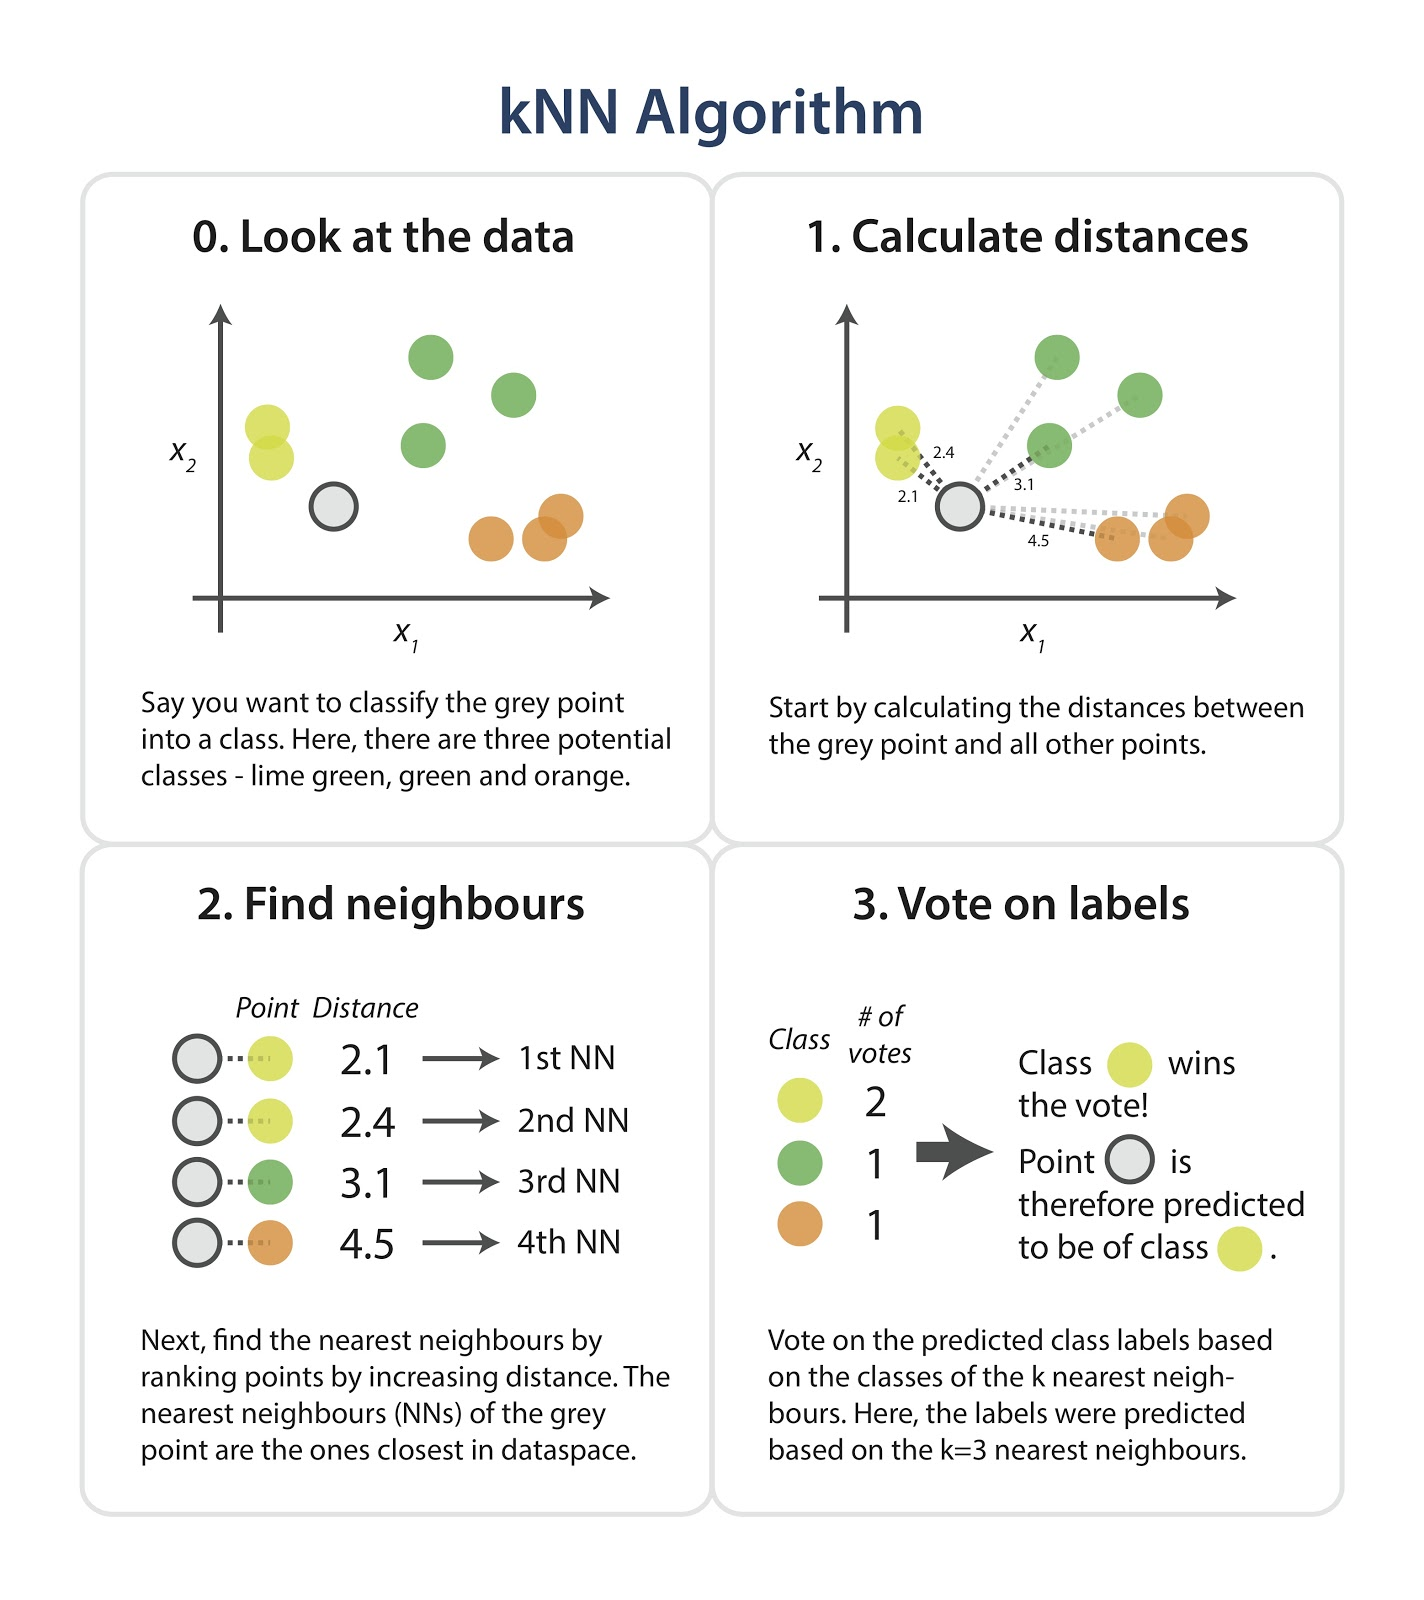
\includegraphics[scale=0.22]{images/knn.jpeg}
%     \caption{Steps of kNN algorithm \citep{knndiagram}.}
%     \label{fig:kNN}
% \end{figure}

% Due to these charactersitics kNNs have been used for astronomical object classfication by \cite{Zhang2012}.
% The hyperparameters in k-nearest neighbours are:
% \begin{itemize}
%   \item \textbf{Number of neighbors (k)}: This hyperparameter determines the number of nearest neighbors in the training data that are considered when making a prediction for a new data point. A larger value of k considers more neighbors, which can smooth out noise but might result in a loss of local detail \citep{sklearn_api}.
%   \item \textbf{Distance metric}: kNN uses a distance metric to measure the similarity or dissimilarity between data points. Common distance metrics include Euclidean distance and Manhattan distance. The choice of distance metric depends on the nature of the data and the problem at hand.
% \end{itemize}



\subsection{Random Forest Classifier}\label{sec:sectionrfc}
The ideology of integrating multiple methods or models to build a predictive model is called ensemble learning methodology\citep{Rokach2010}. Random forests, also known as random decision forests, are an ensemble learning method widely utilized in various domains, including classification and regression tasks. The technique involves constructing an ensemble of decision trees during the training phase. 

In the context of classification tasks, random forests aggregate predictions from multiple decision trees to determine the final class assignment. Each decision tree within the forest independently evaluates a subset of features and a random subset of the training data. By incorporating these randomized components, the random forest fosters diversity among the individual trees, mitigating the risk of overfitting and enhancing robustness.

The underlying principle of random forests centers around the notion that aggregating the predictions of multiple decision trees can yield superior performance compared to any single tree. By combining the outputs of diverse decision trees, the ensemble model is capable of mitigating individual tree biases and errors, resulting in improved generalization and enhanced predictive power \citep{RandomForest1995}.
\begin{figure}[H]
    \centering
    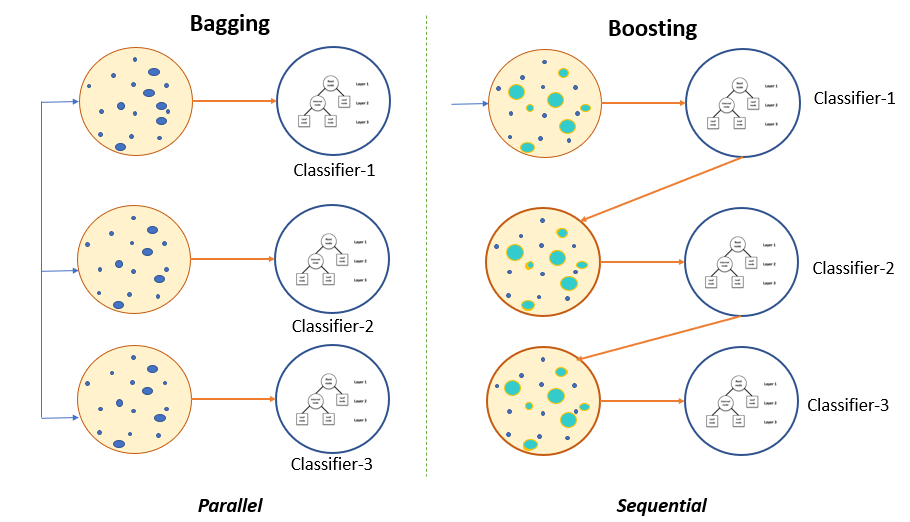
\includegraphics[scale=0.4]{images/bagging vs boosting.png}
    \caption{Bagging vs Boosting \citep{singhal2020a}}
    \label{fig:baggingvsboosting}
\end{figure}
Bagging (Bootstrap Aggregating) is an ensemble learning technique that uses the bootstrap sampling approach i.e., create multiple datasets and train a separate model on each dataset. These models are then combined or aggregated to make predictions in the final ensemble. Bagging technique is commonly used to reduce the variance and improve the overall performance of machine learning model \citep{Breiman2001}. Bagging is employed for two primary purposes. Initially, it is observed that bagging contributes to improved accuracy, particularly when employing random features. Additionally, bagging serves the purpose of continually providing estimates for both the combined ensemble of trees' generalization error, as well as assessments for their strength and correlation \citep{Breiman2001}.

Due to these characteristics random forests have wide applicability in astronomical object classification \citep{Becker2020}.


The important hyperparameters in Random Decision Forests are \citep{scikit-learn}:
\begin{itemize}
  \item \textbf{Number of trees}: Random Forest creates an ensemble of decision trees, and this hyperparameter determines the number of trees in the ensemble. A larger number of trees can improve the model's accuracy but increases the computational cost. If the trees are grown very deep, there is a tendency to learn irregular patterns and overfitting occurs. Random forests take average of multiple decision trees which are trained on different parts of training dataset. This helps in reducing the overall variance and improves the performance of the model. 
  
  \item \textbf{Maximum depth}: This hyperparameter restricts the depth of each decision tree in the Random Forest. Controlling the maximum depth helps to prevent overfitting. A deeper tree can capture more complex relationships in the data, but it may also lead to overfitting if the depth is not properly constrained.
  
  \item \textbf{Number of features}: At each node of a decision tree in Random Forest, a random subset of features is considered for splitting. This hyperparameter determines the number of features to be considered. It provides randomness to the model and reduces the correlation between trees.

  \item \textbf{min\_weight\_fraction\_leaf}: The minimum weighted fraction of the sum total of weights (of all the input samples) required to be at a leaf node. Samples have equal weight when sample\_weight is not provided.
\end{itemize}


\subsection{Gradient Boost Classifier} \label{sec:classifiergbc}

Gradient boosting just like Random forests is another ensemble learning technique. The concept of gradient boosting comes from Leo Breiman's discovery that boosting can be thought of as a way to improve a function by making it better step by step \citep{Breiman2001}. The term boosting originates from the concept of sequentially boosting the performance of a weak learner by focusing on the examples it struggles with. In this context, ``boost'' means to increase or enhance, which reflects the algorithm's objective of improving the predictive power of weak learners \citep{Rokach2010}. The idea behind boosting is to iteratively train new weak learners, giving more attention to the instances that the ensemble struggles to classify correctly. By doing so, each subsequent weak learner ``boosts'' the performance of the overall ensemble by correcting the errors made by the previous learners. \citep{hastie-ch10}

\begin{figure}
    \centering
    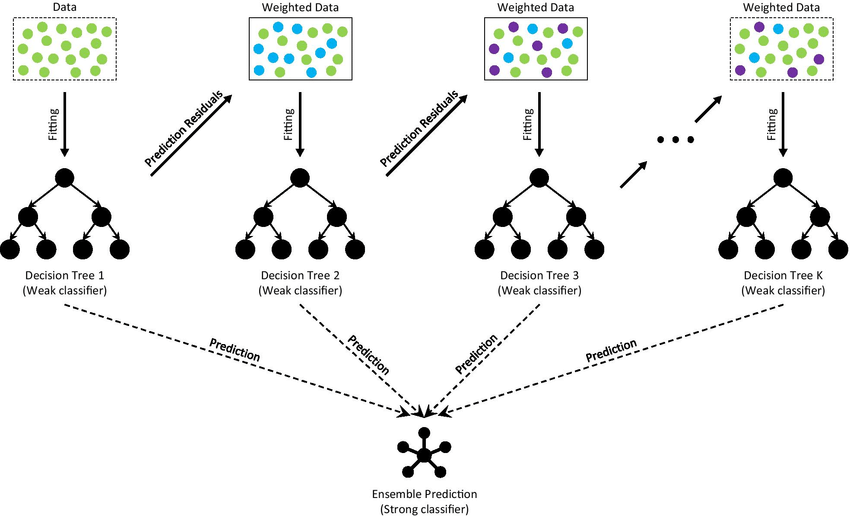
\includegraphics[scale=2]{images/gbc.png}
    \caption{Gradient Boosting in a nutshell \citep{gbcdiagram}}
    \label{fig:gbcnutshell}
\end{figure}



Gradient Boosting assigns weights to the residuals (differences between actual and predicted values) rather than to instances (see \autoref{fig:gbcnutshell}). The algorithm aims to minimize these residuals using gradient descent, iteratively improving the predictions. Gradient Boosting uses various loss functions depending on the problem, such as mean squared error for regression and cross-entropy for classification. The algorithm optimizes these loss functions by minimizing the gradients, hence the name Gradient Boosting \citep{Friedman2001}. The gradient of a function at a specific point is a vector that points in the direction of the steepest increase of that function. In the context of optimization, the gradient points toward the direction in which the function's output increases the most. 



Gradient boosting is working to improve the model's performance by adjusting its parameters in a way that reduces the loss function. To do this, the algorithm utilizes the gradients of the loss function with respect to the model's parameters. By iteratively updating the parameters in the opposite direction of the gradients, the algorithm aims to find the values that lead to the lowest possible loss, thereby improving the model's predictive accuracy.

The hyperparameters in Gradient Boosting Classifier are \citep{scikit-learn}:

\begin{itemize}
    \item \textbf{n\_estimators}: This parameter determines the number of weak learners(trees) to be sequentially added to the ensemble. A higher number generally improves model performance, but it also increases computational cost.

    \item \textbf{learning\_rate}: The learning rate also known as shrinkage or step size, is the parameter that controls the contribution of each weak learner to the ensemble. A lower learning rate makes the algorithm more robust and requires more iterations to converge, but it can prevent overfitting. Conversely, a higher learning rate allows for faster convergence but may lead to overfitting if not controlled properly.

    \item \textbf{max\_depth}: This sets the maximum depth of each weak learner (tree). It controls the complexity of the trees and affects their ability to capture complex relationships in the data.


\end{itemize}

These are a subset of hyperparameters available in a Gradient Boosting Classifier, refer the sklearn GradientBoostingClassifier \citep{sklearn_api} online documentation for a exhaustive list. 

\subsection{Logistic Regression}

Regression techniques are essential in data analysis when you want to understand how one thing depends on others. Linear regression consists of modelling the relationship between a continuous dependent variable and one or more independent variable. The predicted value in linear regression can range from negative to positive infinity, making it suitable for predicting continuous outcomes \citep{hosmerlogisticregression}.

In logistic regression, the outcome variable takes on a binary or dichotomous form, meaning it assumes discrete values. In essence, logistic regression consists of getting the maximum likelihood of an observation belonging to a particular class within a binary classification framework. This technique can be expanded towards estimating probabilities for categorical outcomes, setting it apart from conventional linear regression techniques focusing on predicting continuous numerical values \citep{hosmerlogisticregression}.

The key differences between linear and logistic regression lies in the nature of outcome:

\begin{itemize}
    \item \textbf{Linear Regression:}
        \begin{itemize}
          \item \textbf{Outcome Variable:} Continuous numerical values.
          \item \textbf{Range of Predicted Values:} Can span the entire real number line.
          \item \textbf{Objective:} Minimize the squared differences between predicted and actual values.
        \end{itemize}
        
    \item \textbf{Logistic Regression:}
        \begin{itemize}
          \item \textbf{Outcome Variable:} Binary or categorical values (typically 0 or 1).
          \item \textbf{Range of Predicted Values:} Restricted between 0 and 1, representing probabilities.
          \item \textbf{Objective:} Minimize the log loss (cross-entropy) between predicted probabilities and actual classes.
        \end{itemize}
\end{itemize}

The ``log loss'' (also known as cross-entropy loss) is a mathematical measure used to quantify the difference between the predicted probabilities and the actual classes. It assesses how well the predicted probabilities match the observed outcomes. The main idea is that the log loss is smaller when the predicted probabilities are close to the actual classes and larger when they deviate from the actual classes.

The hyperparameters in Logistic Regression are \citep{scikit-learn}:

\begin{itemize}
    \item \textbf{Cs}: This controls the set of inverse regularization strengths (C values) that the algorithm will consider during cross-validation. Regularization applied to a model refers to the incorporation of a penalty term into the model's optimization process. This penalty term is added to the objective function that the model aims to optimize during training. The primary goal of regularization is to prevent the model from becoming overly complex by discouraging it from fitting the training data too closely. By doing so, regularization aims to improve the model's ability to generalize well to new, unseen data. Regularization helps strike a balance between bias and variance in the model. A model with high complexity (low regularization) can fit the training data very closely, potentially capturing noise in the data. This leads to low bias but high variance, making the model prone to overfitting. Regularization introduces a controlled amount of bias by penalizing complex models, which in turn reduces variance and improves generalization to new data.
    \item \textbf{penalty}: Determines the regularization to be applied in the model. The options are `L1', `L2', `elasticnet', and `None'. L1 regularisation encourages sparsity in the model's coefficients. L2 regularisation prevents large coefficients and reduces overfitting. Elasticnet is the combination of both L1 and L2.
    L1 regularization adds a penalty to the objective function that is proportional to the absolute values of the model's coefficients. Mathematically, it can be represented as the sum of the absolute values of the coefficients. L2 regularization adds a penalty to the objective function that is proportional to the squared values of the model's coefficients. L1 encourages sparsity and feature selection, L2 prevents large coefficients, and Elastic Net combines both techniques to provide a flexible approach that balances their advantages.
    \item \textbf{solver}: Determines the optimisation algorithm to be used to fit the logistic regression model. Some of the options are `newton-cg', `lbfgs' and `sag' which are suitable for multinomial logistic regression. `liblinear' is better for small datasets. In our case we will be using 'saga' (Stochastic Average Gradient descent with Adaptive regularisation) as it is versatile and can handle both L1 and L2 regularisation.
    \item \textbf{max\_iter}: Maximum number of iterations for the optimisation algorithm to converge.
\end{itemize}

This is a subset of key hyperparameters in `LogisticRegressionCV' module of sklearn package. For a full exhaustive list of hyperparameters refer to the official documentation of the LogisticRegressionCV module of the sklearn package \citep{sklearn_api}.


\subsection{Support Vector Machines (SVMs)}
The support-vector network follows the following theory: it maps the input vectors into a high-dimensional feature space using a non-linear mapping that is predetermined in advance. A linear decision surface with unique characteristics is built in this area to ensure the network's excellent generalization ability \citep{SVMCortes1995}. 
Support Vector Machines (SVMs) is a supervised machine learning algorithm used to solve classification and regression problems. The core idea is to find the hyperplane in the feature space to separate two classes \citep{Jin2019}. Like fitting a line in 2D to separate 2 classes, hyperplane separates multidimensional feature space. An optimal hyperplane, see \autoref{fig:svmhyperplane} can be defined as a linear decision function with maximum margin between the vectors of two classes \citep{SVMCortes1995}. 
\begin{figure}[H]
    \centering
    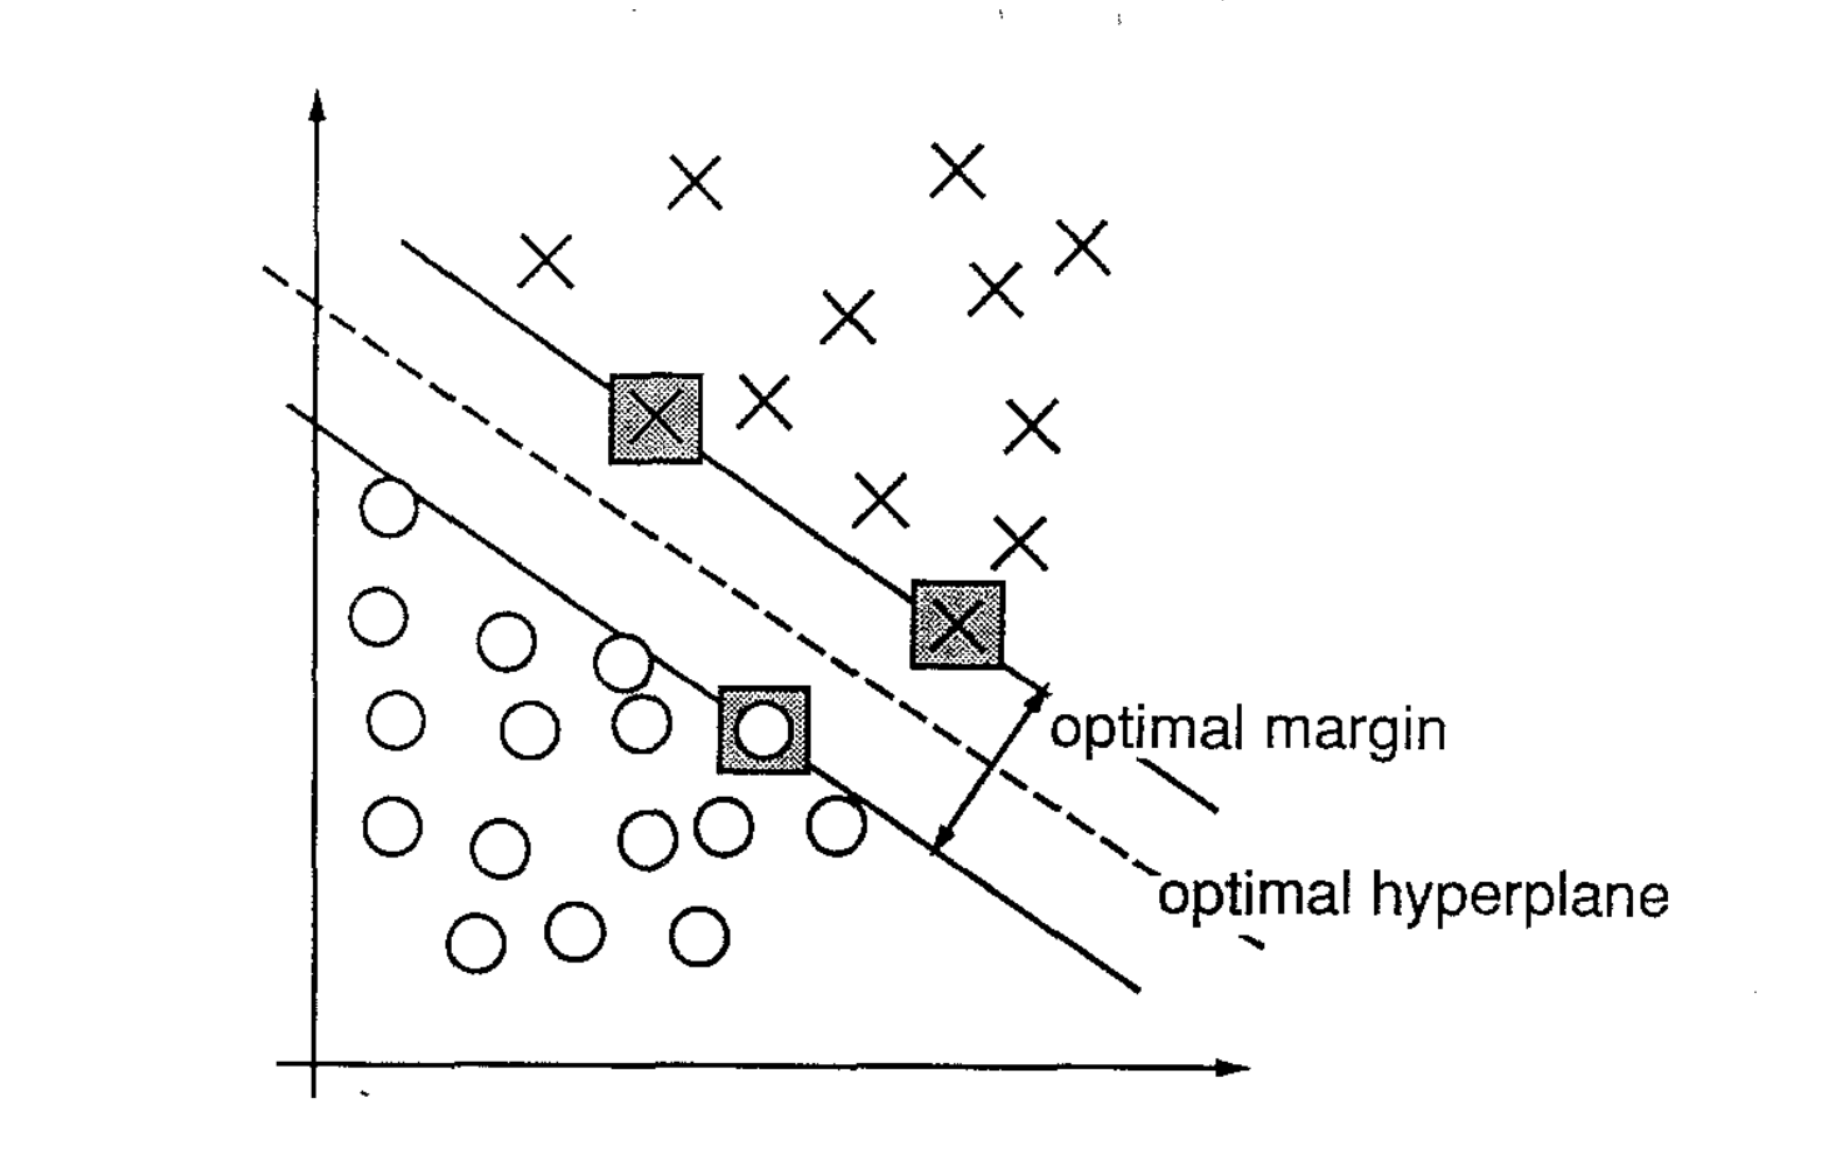
\includegraphics[scale=0.4]{images/SVMHyperplane.png}
    \caption{The support vectors, marked with grey squares, define the margin of largest separation between the two classes \citep{SVMCortes1995}.}
    \label{fig:svmhyperplane}
\end{figure}


One just has to account for a tiny portion of the training data, the so-called support vectors, which define this margin, in order to create such ideal hyperplanes \citep{SVMCortes1995}. SVM has been used widely for classification in astronomy \citep{Zhang2012} \citep{Kim2016}. In SVM, the hyperparameters are, Kernel, C and Gamma \citep{sklearn_api}.
\begin{itemize}
\item \textbf{Kernel}: SVM can use different kernel functions to transform the input data into a higher-dimensional space. The kernel function determines the type of decision boundary created by SVM, such as linear, polynomial, or radial basis function (RBF) kernels.
\item \textbf{C}: This hyperparameter controls the trade-off between maximizing the margin (distance between the decision boundary and the nearest data points) and minimizing the classification errors. A smaller value of C allows more misclassifications but increases the margin, while a larger value of C reduces the margin but minimizes misclassifications.
\item \textbf{Gamma}: This hyperparameter is specific to the RBF kernel and determines the influence of each training example. A higher value of gamma leads to a more complex decision boundary that can fit the training data more precisely. However, it may also result in overfitting if the value is too large.
\end{itemize}


% XGBoost is a boosting algorithm that can be used for classfication and regression problems.  The main difference between XGBoost and Gradient Boost is that Gradient Boost uses the first derivative of loss function to calculate the residual while XGBoost applies first as well as second derivative \citep{Jin2019}. (Need to understand and explain this in more detail)

% Convolutional Neural Networks (CNNs) are a type of neural networks that are good in capturing local and global patterns in input data \citep{Becker2020}. Recurrent neural networks (RNNs) are a family of architecture dedicated to sequential data. These networks can encode information in a fixed-length vector. There features are less biased as they are extracted from the data itself and not designed.\cite{Becker2020} proposed a neural network that can leverage the cast amount of data from the surveys, while reducing the pre processing needed to perform automatic classification. 

\subsection{Cross Validation}
Cross validation is a re-sampling technique which involves partitioning the dataset into subsets (folds), training the model on some folds and evaluating performance on the remaining folds. Cross validation helps to obtain a better estimate of the model's generalisation on new/unseen data. In the K-fold cross validation technique, the dataset is divided into K subsets of roughly equal size. The model is trained K times, each time using K-1 folds for training and 1 fold for validation. The validation fold is then rotated so that every fold gets a chance to serve as the validation set. The performance metrics obtained from each fold are averaged to get an overall assessment of the model's performance \citep{hastie-ch7}.

\begin{figure}[H]
    \centering
    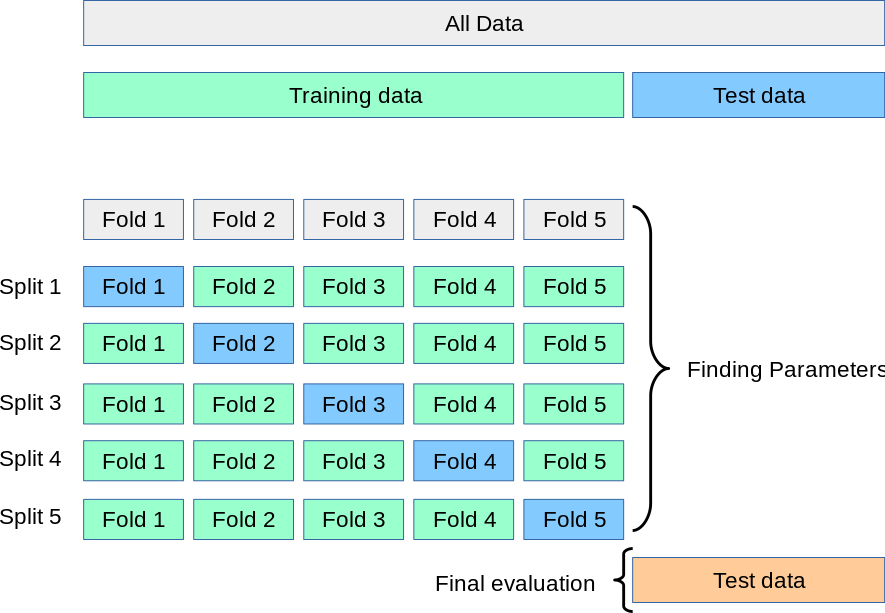
\includegraphics[scale=0.5]{images/cv.png}
    \caption{Example of 5 fold cross validation (K = 5) \citep{scikit-learn-crossval}}
    \label{fig:cv}
\end{figure}

In certain classification scenarios, there's a possibility that the distribution of target classes might be significantly imbalanced. For instance, one class could have far more instances compared to another class. \autoref{fig:classdistribution} shows the class imbalance in the dataset used for this thesis. To address this situation, it's advisable to employ stratified sampling techniques like those provided by StratifiedKFold and StratifiedShuffleSplit. These techniques help maintain the proportional representation of classes in both training and validation sets, ensuring that the relative frequencies of different classes are preserved across the folds \citep{scikit-learn-crossval}. This is important to prevent one class from being underrepresented in the validation set, which could lead to biased evaluation. 


\subsection{Overfitting and Underfitting}

In machine learning, overfitting and underfitting are two common issues that can lead to poor performance of models on new/unseen data. These issues occur when the model is not capable of generalising from the training data.

Overfitting occurs when a model learns data too well which leads to learning underlying patterns as well as noise. This leads to model becoming too complex and fit the training data perfectly but fails to generalise new data. The telltale sign of overfitting is high accuracy on training data but poor performance on validation or test data \citep{Hawkins2004}.
\begin{figure}[H]
    \centering
    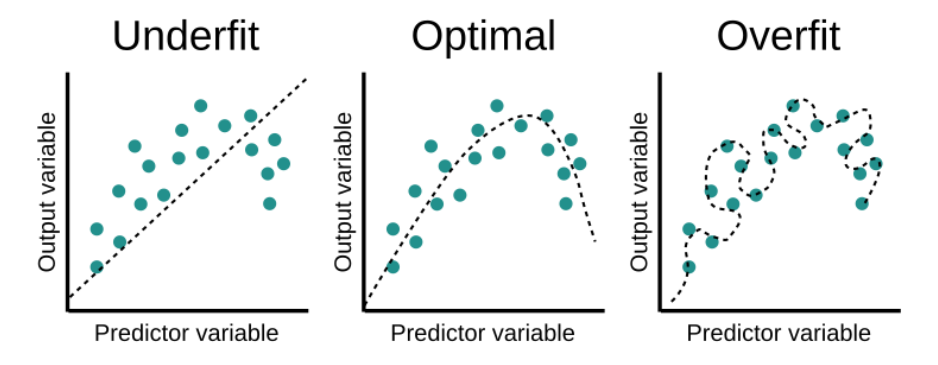
\includegraphics[scale=0.4]{images/fitting.png}
    \caption{Graphical representation of overfit, underfit and good fit \citep{fitting}}
    \label{fig:fitting}
\end{figure}

Underfitting is when a model is unable to adequately learn the training data as well as struggles to make predictions on new data. An underfit model doesn't capture the complexity of the data and misses out on important details and relationships. It may be characterized by low accuracy on both the training and validation/test sets \citep{Hawkins2004}.

The goal in machine learning is to achieve a balanced fit, where the model captures the underlying patterns without being overly influenced by noise. A balanced fit generalizes well to new data, making accurate predictions. To avoid overfitting we can use techniques like regularisation that penalize overly large coefficients which helps of control model complexity. Using cross validation also helps mitigating overfitting. Sometimes gathering more data or increasing the size of data using data augmentation techniques can help the model generalize better. Finding the right balance between model complexity and generalization is a fundamental challenge in machine learning, and addressing overfitting and underfitting is crucial for building effective predictive models.


\subsection{Machine Learning Metrics}
The outputs of machine learning algorithms require careful assessment and this analysis must be interpreted correctly. For this purpose a set of metrics are used to assess the performance of machine learning models. Many metrics are available; however, we will focus on the ones that are commonly used and available in most machine learning frameworks.

\subsubsection{Confusion Matrix}
A confusion matrix is a tabular representation that helps visualize the performance of a classification model by comparing predicted class labels to actual class labels. It's particularly useful for understanding how well the model is doing in terms of true positives, true negatives, false positives, and false negatives \citep{Tharwat2021}.


\begin{itemize}
  \item \textbf{True Positives (TP):} The number of instances that were correctly predicted as positive (correctly classified as the positive class).
  \item \textbf{True Negatives (TN):} The number of instances that were correctly predicted as negative (correctly classified as the negative class).
  \item \textbf{False Positives (FP):} The number of instances that were incorrectly predicted as positive (incorrectly classified as the positive class when they actually belong to the negative class). Also known as a "Type I error."
  \item \textbf{False Negatives (FN):} The number of instances that were incorrectly predicted as negative (incorrectly classified as the negative class when they actually belong to the positive class). Also known as a "Type II error."
\end{itemize}


\begin{table}[h]
\centering
\begin{tabular}{cc|c|c|}
\multicolumn{2}{c}{} & \multicolumn{2}{c}{Predicted} \\
\cline{3-4}
\multicolumn{2}{c|}{} & Positive & Negative \\
\cline{2-4}
\multirow{2}{*}{Actual} & Positive & True Positives & False Negatives \\
\cline{2-4}
& Negative & False Positives & True Negatives \\
\cline{2-4}
\end{tabular}
\caption{Confusion Matrix}
\end{table}

\subsubsection{Accuracy}
Accuracy is defined as the ratio of correct predictions to the total number of predictions. It is the most common metric used to evaluate performance of a machine learning algorithm. It provides a general overview of model's correctness but it is not robust as imbalanced classes can give misleading accuracy scores \citep{Tharwat2021}.

\begin{equation}\label{eq:acc}
    Acc=\dfrac{TP+TN}{TP+TN+FP+FN}
\end{equation}

\subsubsection{Precision}
Precision also referred to as \textit{Positive prediction value (PPV)}, is defined as the ratio of true positive predictions to the total number of positive predictions. This metric is also affected if the data is imbalanced \citep{Powers2008}.

\begin{equation}\label{eq:precision}
    PPV=Precision=\dfrac{TP}{FP+TP}
\end{equation}

\subsubsection{Recall}
Recall also referred to as \textit{True positive rate (TPR)} or \textit{Sensitivity} is defined as the ratio of true positive predictions to the total number of actual positives. This metric is relevant when false negatives predictions are risky especially in the field of medicine. High recall indicates that the model is capturing most positive instances correctly \citep{Tharwat2021} \citep{Powers2008}.

\begin{equation}\label{eq:recall}
    Recall = \dfrac{TP}{FN+TP}
\end{equation}

\subsubsection{F1 Score}
The F1-score, often used in machine learning for classification tasks, is defined as the harmonic mean of precision and recall. In mathematics, the harmonic mean is a type of average that's particularly useful when dealing with rates or ratios. F1-score ranges from zero to one and high value can be interpreted as good classification performance \citep{Powers2008}. 

Harmonic mean is calculated by taking the reciprocal of the arithmetic mean of the reciprocals of a set of values. The formula for the harmonic mean of values $x_1,x_2,x_3...x_n$ is:

\begin{equation}\label{eq:harmonic}
    H=\dfrac{n}{\frac{1}{x_1}+\frac{1}{x_2}+\cdots+\frac{1}{x_n}}
\end{equation}

Using equations for precision and recall - \autoref{eq:precision} and \autoref{eq:recall} we can write the equation for F1-score using the equation for Harmonic mean \autoref{eq:harmonic}:

\begin{equation}
    \label{eq:f1}
    F_1 = \dfrac{2}{\frac{1}{recall}+\frac{1}{precision}}=2\cdot\dfrac{precision\cdot recall}{precision+recall}= \dfrac{2TP}{2TP+FP+FN}
\end{equation}

F1-score balances precision and recall, giving a single score that considers both false positives and false negatives \citep{Tharwat2021}.

\subsubsection{Logloss}

Logarithmic Loss, commonly known as Log Loss or Cross-Entropy Loss, is a widely used evaluation metric for classification problems, particularly in scenarios where the model's predicted probabilities are important. It measures the performance of a classification model by quantifying the difference between predicted probabilities and actual class labels. Log loss values range from 0 to positive infinity with lower values indicating better model performance. Log loss heavily penalizes incorrect high-confidence predictions. If a model assigns high probabilities to incorrect classes, the log loss will increase substantially \citep{sklearn_api}.




% ------------------------------------------------------------------------------------------

\section{Genetic Algorithms (GAs)}
According to Darwin's rule of natural selection, organisms with phenotypes that are well matched to their immediate environment will eventually have a higher probability of reproducing and/or surviving than other, less suitable species \citep{DODSON1976243}. Phenotype refer to the observable physical and behavioral characteristics of an organism, resulting from the interaction between its genetic makeup (genotype) and its environment. In the following generations, only those phenotypes prevails which are more suited to the environment. Mutation of genes can cause the organism to either have better characteristics or worse characteristics. But natural selection will eventually carry forward those mutations which are better.\par
Genetic Algorithm (GA) is a computational model which takes inspiration from Darwin's law of natural selection. The terminologies used to describe such types of algorithms are analogous to the biological ones. A population-based search technique called the Genetic Algorithm (GA) creates new populations by repeatedly using genetic operators or randomization functions \citep{Katoch2021}. GA effectively searches an encoded parameter space by using the objects from the population and the randomization technique \citep{Liu2019}.

A population is initialized using random variables (traits/characteristics), a set of variables is referred to as chromosomes. The main components of GA are chromosomal representation, crossover, fitness selection,  mutation, and fitness function computing. Until off-springs generated provide the ideal solution or the maximum number of iterations is achieved, the selection, crossover, and mutation procedures on the population are repeated. GA can be summarised in the form of a pseudo-code. \par



The fundamental theorem of GA is the Schema Theorem \citep{Liu2019}. ``According to Schema theorem, the original schema has to be replaced with modified schema. To maintain the diversity in population, the new schema keeps the initial population during the early stages of evolution. At the end of evolution, the appropriate schema will be produced to prevent any distortion of excellent genetic schema." \citep{Katoch2021} The most crucial element of genetic operators is the crossover operation. It is a recombination operator that joins pieces of the chromosomes of two parents to create offspring that have a portion of both parents' genetic makeup. \citep{Tang1996}. ``The offspring generation formed by the cross-interchange of the parental chromosomes is likely to discard or destroy the excellent genetic schemas possessed by the parental individual."\citep{Liu2019} \par

% url = {https://www.sciencedirect.com/science/article/pii/0025556476901279},

\subsection{Genetic Operators}\label{sec:geneticoperators}
Genetic operators are the operators that are used during the optimisation process. See \autoref{fig:GAOperators} the general operators are encoding schemes, selection, crossover and mutation. 

\begin{figure}[H]
    \centering
    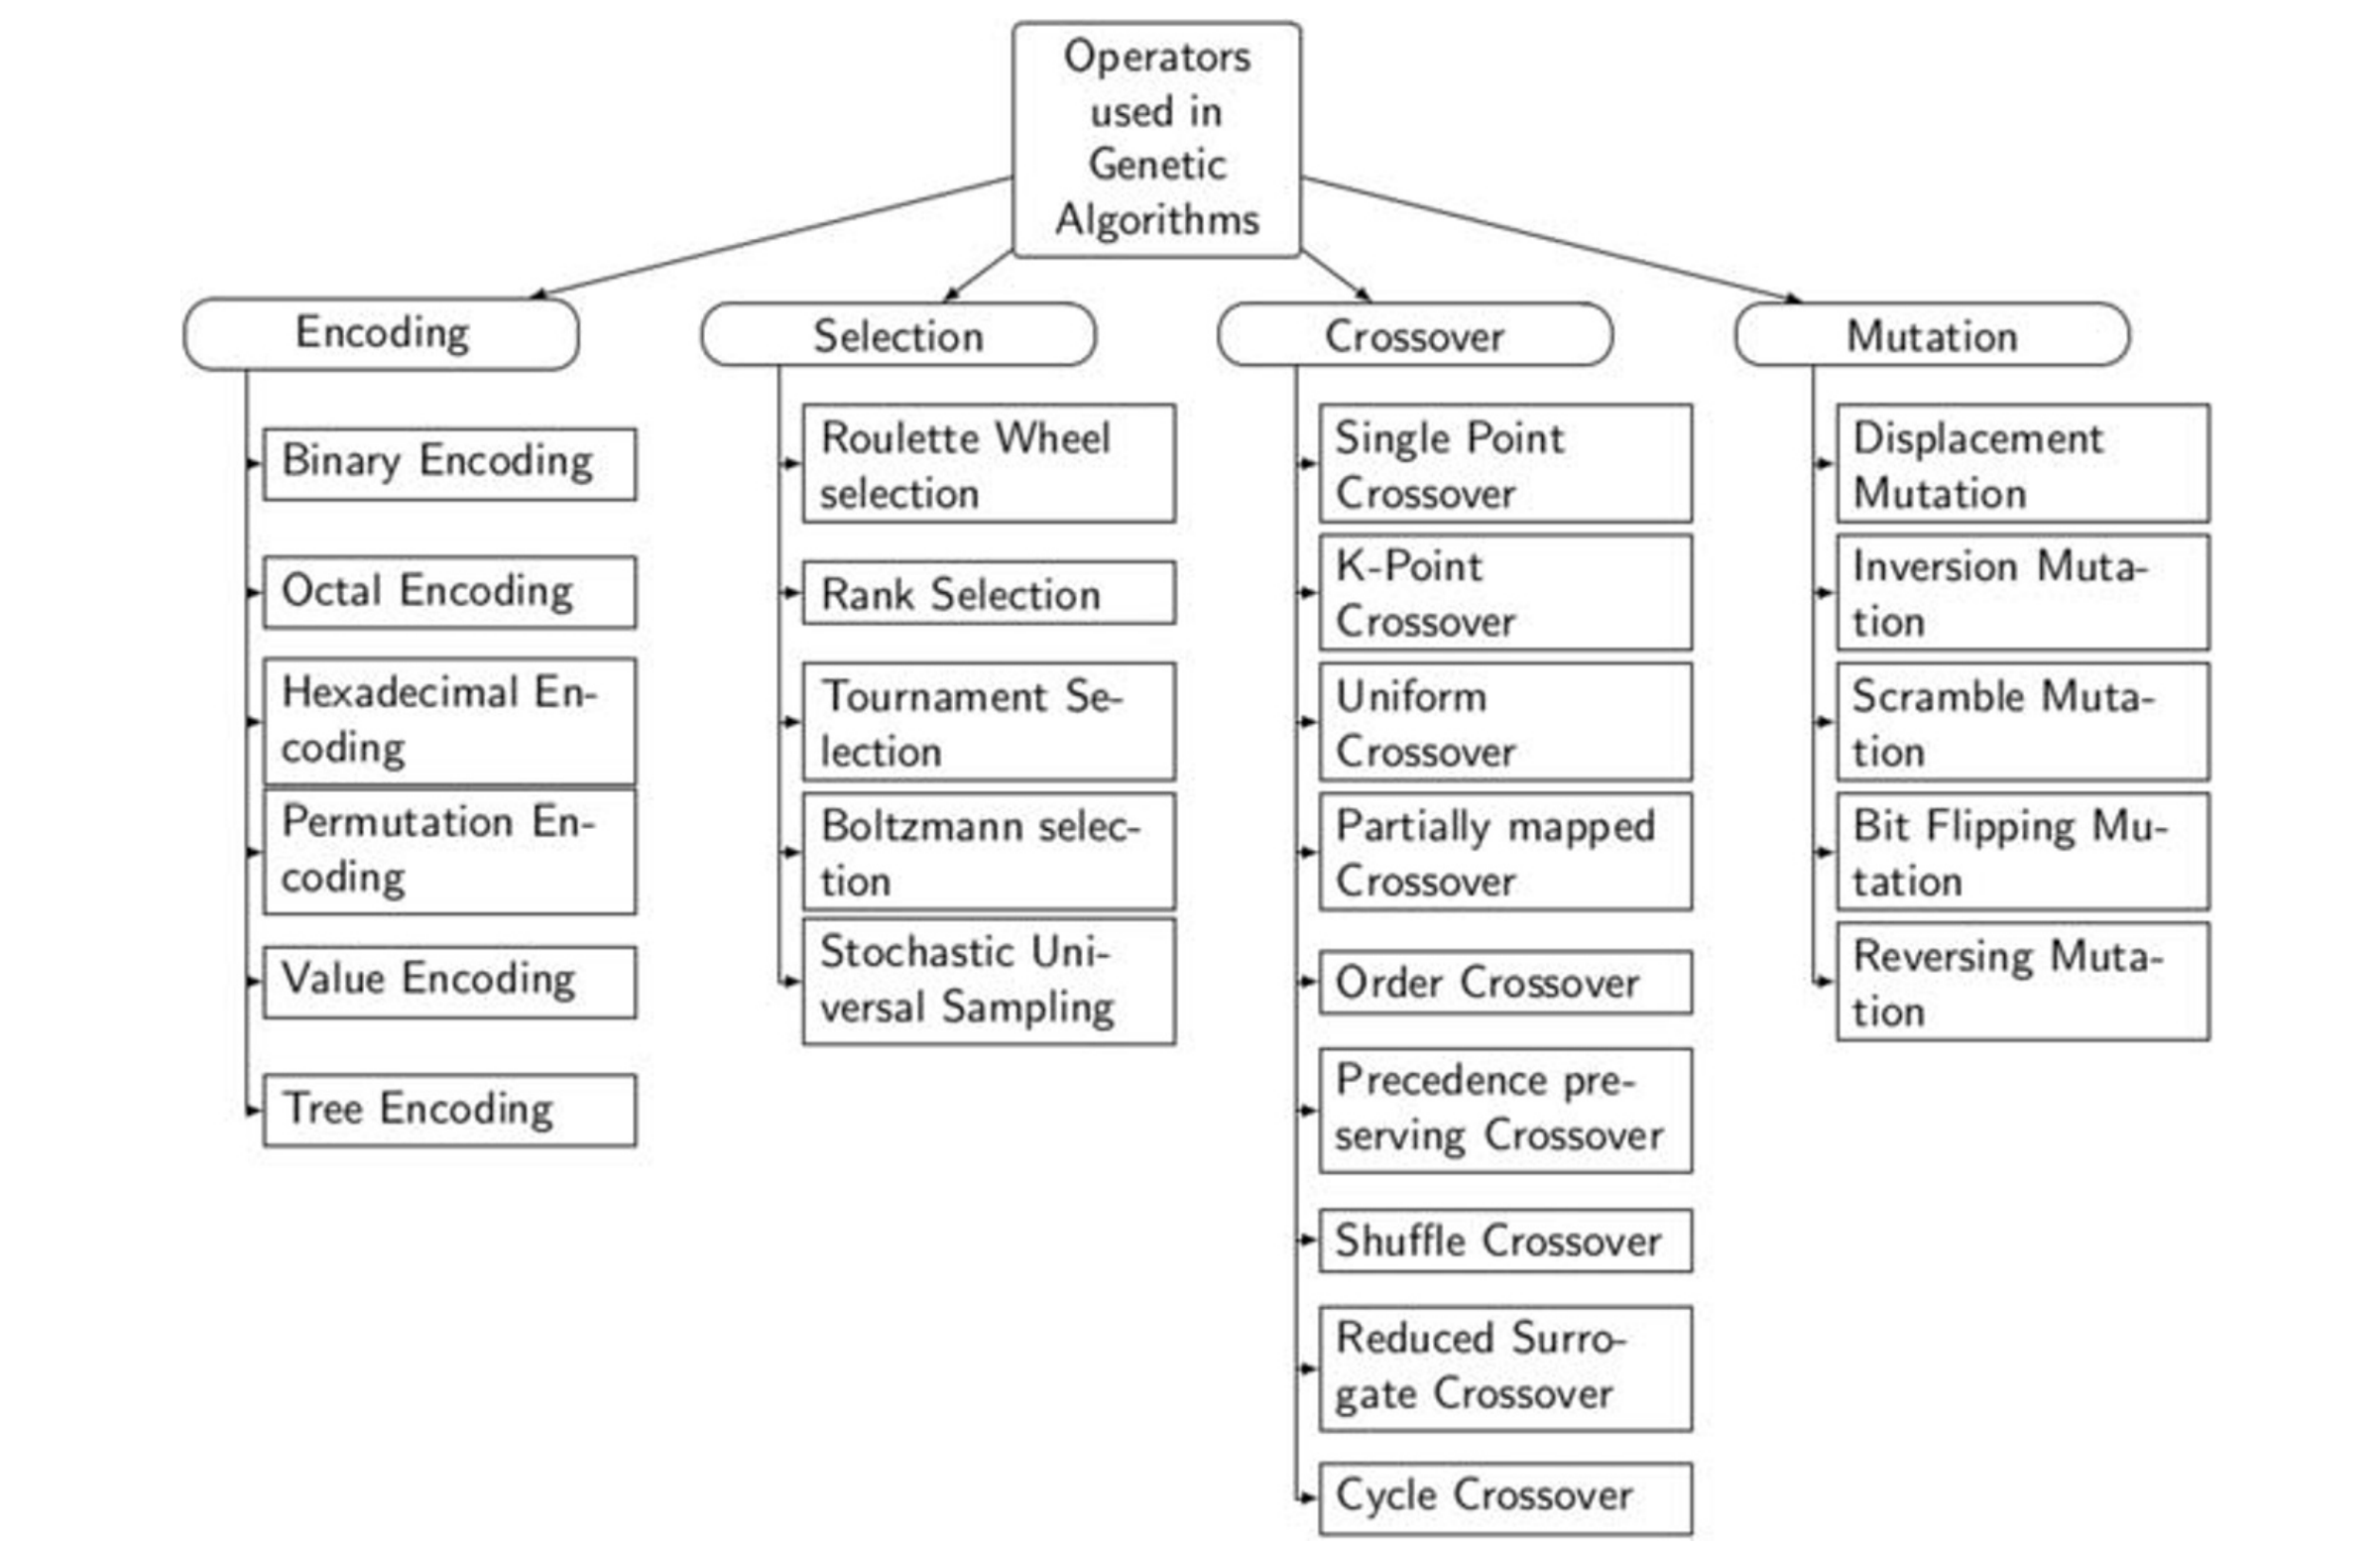
\includegraphics[scale=0.4]{images/GA_Operators.png}
    \caption{Operators used in Genetic Algorithms \citep{Katoch2021}}
    \label{fig:GAOperators}
\end{figure}

\subsubsection{Representation (Encoding Schemes)}
We encode the solution set of the problem to improve the algorithm's performance. This encoded object functions analogous to a chromosome. It is not the problem in itself, but rather a collection of attempted solutions to the problem. The chromosome can be represented / encoded as binary, octadecimal, or hexadecimal values, and these can then be subjected to crossover and mutation to provide a more likely set of solutions. Aside from numerical encoding, ``permutation encoding" is generally preferred in ordering problems.

\subsubsection{Selection}
In genetic algorithms, selection is a key phase that determines whether  a particular string participates in reproduction. Boltzmann, rank, tournaments, roulette wheels, and  universal probabilistic sampling are examples of well-known selection techniques. The roulette wheel selection method maps all possible strings to the wheel and assigns each string a space on the wheel  based on the fit value. This wheel is then randomly rotated to select a specific solution involved in building the next generation \citep{Holland} \citep{Katoch2021}. \par
The modified version of roulette wheel selection is ranked selection. Instead of using fitness value, it uses rankings. Brindle introduced the tournament selection approach in 1983, in which the individuals are chosen in pairs from a stochastic roulette wheel based on their fitness scores. Following selection, those with a greater fitness value are added to the pool of the following generation. \citep{Holland}\par
The existing roulette wheel selection method is extended by stochastic universal sampling (SUS). It chooses an individual at regularly spaced intervals from a list of individuals from a generation, starting at a random position. All individuals have an equal chance of being chosen to take part in the following generation's crossover \citep{Katoch2021}.

\subsubsection{Crossover}
In order to create offspring, crossover operators combine the genetic information of two or more parents.

% The crossover formula is given as: 
% \begin{equation}
%     R = \frac{\left(G + 2 \sqrt{g}\right)}{3G}
% \end{equation}

% where $\mathbf{G}$ is the total number of evolutionary generations that have been set for this population in advance, and $\mathbf{g}$ is the amount the algorithm has ran for number of generations \citep{Liu2019}. \par
Many GA practitioners believe that the crossover operator is what really sets the GA apart from all other optimization algorithms. There are several crossover operation variants offered, with a single-point crossover being the most basic. Based on the selection methodology, the parents are randomly chosen. The regions of the two chromosomes beyond the crossover point are exchanged to create the offspring, where the crossover point is determined by a random process \citep{Tang1996}.\par
Similar to single-point crossover, multipoint crossover uses m crossover sites that are randomly selected without duplication. The crossover operator that is most often employed is partially matched crossover (PMX). This operator outperforms the majority of the other crossover operators in terms of performance \citep{Katoch2021}.

\subsubsection{Mutation}
An operator that modifies the chromosome is called mutation. The mutation can take place both on a global and local level. The procedure randomly changes the value of a string position occasionally (and typically with low probability $p$) \citep{Tang1996}. The three most well-known mutation operators are scramble mutation, simple inver-sion, and displacement.\par

The scramble mutation (SM) operator arranges the components of each individual solution in a random order and determines whether the freshly created solution's fitness value has increased or decreased \citep{Jebari}.

The SIM (simple inversion mutation operator) inversion operator flips the randomly chosen string and positions it in a random spot. Between any two given places in a single solution, the substring is reversed using the SIM \citep{Jebari}. 

The displacement mutation (DM) operator moves an individual solution's substring within itself. To ensure that both the final solution and a random displacement mutation are legitimate, the location is randomly selected from the substring that is being used for displacement. Exchange mutation and insertion mutation are two types of DM variations. A portion of a unique solution is either swapped with another portion or inserted in a different position in exchange mutation and insertion mutation operators, respectively. \citep{Jebari}\par

\section{Tools and Technologies}

This section will include all the tools and technologies that I used for the thesis with a breif description. The choice of programming language is Python due to its extensive documentation, open source nature and availability of sophisticated packages. For the workflow the choice of platform was Jupyter notebook (formerly IPython Notebook) which is an interactive way to write blockwise code. Due to its versatile nature it is a great tool for experimentation. 
Here are some key features of Jupyter notebooks:

\begin{itemize}
    \item Interactive Execution: Jupyter Notebooks allow you to execute code cells interactively. Each code cell can be executed individually, and the results are displayed directly below the cell. This interactive nature enables users to experiment with code, test hypotheses, and observe immediate outcomes.
    
    \item Mixed Content: Notebooks support not only code but also markdown cells for rich-text formatting, \LaTeX equations, images, links, and explanatory text. This combination of code and narrative makes it an effective tool for presenting and documenting analysis processes and findings.
    
    \item Visualization: Notebooks can display visualizations, graphs, and charts inline with the code, enhancing the ability to understand data patterns and relationships.
    
    \item Step-by-Step Exploration: Jupyter Notebooks encourage a step-by-step exploration of data and algorithms. By breaking down tasks into smaller blocks of code and text, it becomes easier to understand the logic behind each step.
    
    \item Reproducibility: Notebooks promote reproducible research by documenting code and results in a single document. This enables others to reproduce your work and verify your findings.
    
    \item Interactivity: Besides code execution, notebooks can incorporate interactive widgets and dashboards using libraries like ipywidgets. This enables dynamic manipulation of parameters and variables, enhancing the user's engagement with the content.
    
    \item Sharing and Collaboration: Jupyter Notebooks can be shared easily by exporting them to formats like HTML, PDF, and slides. They can also be hosted on platforms like GitHub, allowing others to view and interact with your analysis.
    
    \item Kernel Support: Jupyter Notebook's kernel architecture allows you to connect to different programming languages. This enables users to work with multiple languages within a single notebook.
    
    \item Educational Tool: Jupyter Notebooks are extensively used in educational settings to teach programming, data analysis, and scientific computing. The combination of code, explanations, and visualizations makes learning concepts more engaging.
\end{itemize}

Some of the Python libraries that were used for the data analysis and machine learning are:
\begin{itemize}
    \item \textbf{NumPy}: Used in data analysis for numerical python which uses N dimensional array objects for mathematical operations \citep{NUMPY}.  
    \item \textbf{Pandas}: Used mainly for working with relational or labelled datasets. It is based on NumPy increasing its efficiency and making it suitable for statistical analysis \citep{PANDAS}.
    \item \textbf{Matplotlib}: The primary plotting library in python with extensive community support \citep{MATPLOTLIB}.
    \item \textbf{sklearn}: Machine learning library which provides all the necessary functionality right from preprocessing of data to evaluation of machine learning model performance. Detailed documentation with good community support makes it a very useful library for machine learning applications \citep{scikit-learn} \citep{sklearn_api}.
    \item \textbf{sklearn-genetic-opt}: Sklearn-genetic-opt uses evolutionary algorithms from the deap package to choose a set of hyperparameters that optimizes (max or min) the cross-validation scores, it can be used for both regression and classification problems.
\end{itemize}

For keeping track of research papers and citations I used Mendeley reference manager \citep{Mendeley}. It is a tool that can extract relevant metadata - authors, title, year, journal, volume, issue etc using the DOI (Data Object Identifier) number of published research papers, conference proceedings, books, reports, journal articles, etc. The reference manager allows to read paper, make notes, highlight text in research papers and many other features useful for literature review. Mendeley reference manager also allows you to create a collection of research papers and export the bibliography file with all the metadata in multiple formats. \LaTeX was the choice of type setting format for writing the thesis as it is the best in class used to produce publication quality documents. \LaTeX (pronounced "lay-tech" or "lah-tech") is a typesetting system commonly used for creating documents with complex formatting, such as academic papers, research articles, theses, reports, books, and presentations. It is particularly popular in the fields of mathematics, computer science, engineering, and academia in general. LaTeX allows you to produce high-quality documents with consistent and professional-looking layouts, equations, tables, and references. The exported .bib file from mendeley can be used to add citations easily while writing the document. Final document was written on overleaf which is a cloud \LaTeX compiler as it is safe to have these files on cloud with version control. 